% !TEX root = ../thesis.tex
\chapter{绪论}
本章首先介绍了数据驱动的相似性学习的研究背景,然后讨论了数据驱动的相似性学习相关的研究现状,最后本章介绍了本文的重要贡献以及后续章节的内容安排。
\section{研究背景}
随着机器学习、数据挖掘、计算机视觉等研究方向下计算机技术的高速发展,通过“图”\cite{chung1997spectral}表示的结构化数据分析一直是人工智能领域的核心问题之一。本文所研究的数据驱动的相似性学习方法则立足于图结构下的数据建模。因此本节将首先介绍图结构基本概念,然后对图方法的一些典型应用进行介绍,最后介绍在具有图结构的数据中进行相似性学习的研究意义。

在部分机器学习的实际应用场景中,数据样本通常是以独立个体的形式存在,例如大规模图像分类任务、目标检测任务或图像生成任务。但在大量的机器学习应用中,数据是以相互关联的形式存在,例如社交网络分析中用户间的关联性、图像分割中邻近的不同像素之间的联系以及论文数据之间的引用关系等。即使在图像生成任务中,也可以通过考虑生成图像不同像素区域间的相似性关系在一定程度上提升所生成图像的保真度\cite{zhang2018self}。对于这种数据之间存在强关联性的数据分析问题,可以在机器学习的过程中引入图论中的图结构对数据本身及数据之间的关联进行抽象建模,并利用谱图理论(spectral graph theory)\cite{chung1997spectral}或信息传播对所需的图上信息进行学习及推理。

通常情况下,图方法将数据中的每个数据实例视作图中的顶点(vertex),将数据之间的存在的连接性用图上边(edge)表示,根据不同的应用场景该顶点可以为社交网络中的一个用户、分子结构中的一个原子、一张图像或图像中的一个超像素等。在该抽象模型下,若在共有$n$个实例的数据集$\mathcal{X}=\{x_1,\dots,x_n\}$中实例$x_i$与$x_j$存在被观测到连接性,则顶点$x_i$与$x_j$之间存在边$e_{ij}=(x_i, x_j)$。所有边构成边集$\mathcal{E}=\{e_{ij}|x_i, x_j\in \mathcal{X}\}$,则相应的图可以被表示为$\mathcal{G} = (\mathcal{X}, \mathcal{E})$。此处不对第$i$个抽象数据实例及其对应的数据观测特征进行区分,均采用$x_i$表示。若在观测到两个实例是否存在关联之外,同时可以观测或构造出顶点之间的相关程度大小,则该数值可以以边$e_{ij}$上的权值(weight)$w_{ij}$表示,一般也被称为数据间的相似性(affinity)。在不同的数据集和应用场景下,该图可以为无向图或有向图。在仅观测到连接性而无法观测或构造出数据实例间相似性的情况下,可以采用二值的邻接矩阵(adjacency matrix)$A\in\mathbb{R}^{n\times n}$表示数据之间的邻接关系。对于$A$中元素$a_{ij}$,若$e_{ij}\in \mathcal{E}$则$a_{ij}=1$,否则$a_{ij}=0$。在能够获取到数据间相似性的情况下,可采用相似性矩阵(affinity matrix)$W\in\mathbb{R}^{n\times n}$表示成对数据之间的相似性,若$e_{ij}\in \mathcal{E}$则$w_{ij}>0$,否则$w_{ij}=0$。在部分特定领域应用下,存在边具有不同类别或具有特征描述的情况,以及存在包含不同类型顶点的异构图(heterogeneous graph)情况。本文将重点讨论仅考虑相似性矩阵$W$及顶点集$\mathcal{X}$的情况,则对应的图也可被表示为$\mathcal{G} = (\mathcal{X}, W)$。

图方法其本身既可以直接用于监督或半监督的顶点分类\cite{kipf2016semi,velivckovic2017graph,hamilton2017inductive}、无监督的图嵌入\cite{roweis2000nonlinear,belkin2001laplacian,perozzi2014deepwalk,kipf2016variational}、图分类\cite{shervashidze2011weisfeiler,defferrard2016convolutional,zhang2018end,xu2018how}及图生成\cite{simonovsky2018graphvae,de2018molgan,li2018learning}等抽象任务,也可以作为结构化信息传播的方法用于大量具体任务。在计算机视觉方面,图方法既可以用于以单个图像作为顶点的任务上,如:小样本学习\cite{garcia2018fewshot}、图像聚类\cite{blaschko2008correlational}、图像哈希\cite{weiss2009spectral}等,也可以用于以图像及特征中的像素或超像素为顶点的任务,如:视频动作识别\cite{wang2018non}、图像语义分割\cite{huang2019interlaced}、图像描述\cite{yao2018exploring}、无语义分割\cite{shi2000normalized}、3D点云\cite{wang2019dynamic}、自然图像抠图\cite{levin2008closed}、深度估计\cite{cheng2018depth}及图像补全\cite{yu2018generative}等。此外图方法还广泛应用于自然语言处理\cite{vaswani2017attention}、分子结构分析\cite{kearnes2016molecular}、推荐系统\cite{ying2018graph}及社交网络\cite{hamilton2017inductive}等领域。本文将重点关注于图方法中相似性学习在计算机视觉方向上的应用。


多数图方法采用给定或观测到的图结构及相似性权重,而不是通过数据对相似性进行学习。在图结构中进行相似性学习的研究主要有两个方面的意义。
一方面在于,若所获取的数据虽然应具有潜在的结构信息,但数据间的关联性却无法被直接观测到,则需要对相似性进行启发式构造或学习。另一方面在于,通常观测到的或启发式方法构造出的相似性矩阵与后续学习任务是两个分离的阶段,所获取到的相似性信息对于实际的学习任务可能不是最优的或存在噪声信息,因此可以通过数据驱动的相似性学习获取更优的相似性信息。例如,在社交网络数据集Reddit\cite{hamilton2017inductive}中,若同一个用户同时评论了两个不同的帖子,则两个帖子之间将建立边进行关联。但在实际场景中,同一用户存在较大概率会在不同类别的帖子上发出评论引入噪声边,相对的,帖子本身的词向量特征也可以用于学习数据之间的相似性,对已有的边进行调整。
相似性学习既可以以归纳式(induction)的方式学习出从数据到相似性的通用映射函数\cite{meila2001learning}也可以采用优化等转导式(transduction )方法直接通过观测数据学习到相似性信息\cite{nie2014clustering}。

\section{研究现状}

目前相似性学习存在的问题及难点主要为两个方面,一方面在于所采用的数据信息能否支撑相似性学习,另一方面在于相似性学习本身可扩展性较差。

对于第一方面问题,在数据驱动的相似性学习中往往存在所用的信息无法支撑所需相似性生成的问题。在部分场景下,所观测到的数据实例之间虽然存在潜在的图结构上的相似性,但所观测到的数据特征中无法对该相似性进行体现,即我们无法通过观测到的数据或其特征符合逻辑地构造数据实例间的相似性关系。例如在社交网络中若仅观测到用户发布的照片信息,虽然可以以此计算不同用户间的共性,但却无法正确建立用户与用户间的社交关系。在假设所观测数据足以支撑相似性生成的前提下,依然存在的一个问题是如何从数据中提取可以有效学习相似性的信息。部分基于深度学习的文献通过计算其任务特征间的相似程度作为相似性\cite{velivckovic2017graph,wang2018non},即在单一网络的端到端预测任务中抽取网络中间的特征作为相似性计算的依据。对于所需相似性与待预测信息具有一致性的情况下该策略可以取得较好的效果,例如在视频动作识别中用语义特征使不同图像帧之间相同的物体或部件产生关联\cite{wang2018non}。但在图像抠图等低级图像处理应用中,图像纹理特征间的关联性可能相对于语义特征更加重要,因此需要进行独立的学习。

对于第二方面,如果需要对不存在图结构的数据顶点进行数据驱动的图上相似性学习,即通过数据实例构造边以及边上的相似性权重,为不遗漏可能存在的相似性,一般需要对任意一对顶点间的关系进行考察。该穷举式的学习预测过程的复杂度在$O(n^2)$以上,仅能处理数据量有限的小数据情况,而对大数据则难以扩展。相对于完整的图结构构造,在已知图结构的数据上仅学习相连接数据间的相似性则具有更高的学习效率,可以将复杂度降至$O(|\mathcal{E}|)$。此外,如对现有图结构进行更新或采样获取新的图结构等思路则更具有灵活性,其复杂度也大致在可接受范围内。

若将二值邻接矩阵及具有多种边类别的邻接矩阵均看作相似性的扩展形式,则目前的相似性学习大致分为三类:

\begin{itemize}
    \item {\bf{确定图结构下的相似性学习}}。
    自注意力机制\cite{vaswani2017attention,wang2018non}本身可以看作完全图上的相似性学习,相应的GATs方法\cite{velivckovic2017graph}则可以根据其输入的图结构对已知边上的相似性进行学习。
    而稀疏自注意力机制\cite{child2019generating,huang2019interlaced}或局部自注意力\cite{ramachandran2019stand}则可以认为是根据图像结构特性所构造的稀疏图上的相似性学习方法。
    此外SPN\cite{liu2017learning}及CSPN\cite{cheng2018depth}方法通过一个辅助网络对图像中的空间近邻点间的相似性进行学习,并将预测出的空间局部相似性作用于主网络中,对特征信息进行迭代扩散,实现空间上信息传播的效果。
    ECC方法\cite{simonovsky2017dynamic}采用辅助网络的方式以边的标签作为输入,动态生成边上的滤波器参数,能够同时实现图上顶点特征的变换和聚合,该方法可以看作相似性学习的一个扩展形式,且其所生成的边上参数仅依赖边的标签而不依赖于顶点特征。文献\parencite{kearnes2016molecular}利用成对顶点的特征对边特征进行更新,也可以认为是相似性学习的一个特例。    
    \item {\bf{对已知图结构的调整}}。
    文献\parencite{pavan2007dominant}提出在已知图上选择最大团的方式对现有图结构进行优化,删除噪声边,获取更稳定的图连接。
    Wang等人在文献\parencite{wang2009unified}中通过学习凸组合系数的方式,基于多个不同模态下的已知图结构学习出融合后的相似性矩阵。文献\parencite{premachandran2013consensus}提出采用二阶相似性的思路,对已知图结构上相互连接的点对统计公共近邻顶点数量,以此为标准剔除噪声边。
    AffinityNet\cite{ahn2018learning}在弱监督分割问题上采用了更灵活学习方式,其通过在输入图像上采样具有监督信息的边,以训练一个对任意像素点对可用的相似性预测网络,而在预测网络训练完成后仅根据像素坐标位置对相邻像素点进行连接,构造局部相似性。    
    \item {\bf{图结构生成}}。由于从零开始对数据生成图结构具有极高的复杂度,除了少数复杂度较高的算法外多数方法会将应用限制在顶点数量极少的场景下,例如:有机分子结构生成或图像中物体关系生成。
    文献\parencite{meila2001learning}提出通过监督数据学习出一个从边的特征到顶点间相似性的非线性映射函数,并将其用于图像分割问题。
    Nie等人在文献\parencite{nie2014clustering}中提出根据数据特征间的距离通过优化的方式获得任意数据点对之间的相似性,并通过稀疏约束以获得自适应的非完全图结构,将该优化问题与谱聚类合并则可以实现在谱聚类过程中同步实现图结构生成。
    MolGAN\cite{de2018molgan}结合生成对抗网络\cite{goodfellow2014generative}及图卷积网络\cite{kipf2016semi}用于有机分子生成。GraphVAE方法\cite{simonovsky2018graphvae}通过结合ECC模型\cite{simonovsky2017dynamic}的网络结构与变分自编码器,对特定标签的有机分子结构进行生成。文献\parencite{li2018learning}通过时序模型以无顶点的空图为起点依次生成顶点及边,构造分子结构。文献\parencite{yao2018exploring}将边的类别学习用于在图像描述(image caption)生成问题中建立图像中物体的联系,其通过一个单独的网络对图像中目标物体对之间的关系进行分类,用于构造图卷积网络中的语义图。
\end{itemize}


\section{本文主要工作及贡献}
在本文中,我们从无监督度量学习的图像聚类、半监督的多模态约束聚类及监督学习下的图像抠图三个方面对数据驱动的相似性学习在计算机视觉问题中的应用进行了研究。希望能够通过所提出的相似性学习方法,在不同的基于图结构的计算机视觉应用问题上产生相应的贡献。
% 本文的主要研究工作及贡献包括以下三个方面:无监督度量学习下的图像聚类、半监督的多模态约束聚类及监督学习下的图像抠图。

\subsection{无监督度量学习下的图像聚类}
在无监督图像聚类中,基于图结构的图嵌入聚类算法往往会通过启发式方法建立数据间的相似性矩阵(affinity matrix)以描述图像间的相关联程度,并基于此相似性矩阵实现不同的优化学习方法。由于数据本身噪声等原因,基于启发式方法获得的相似性矩阵本身具有不稳定,可能会导致不同类别下外观相似的图像之间存在较大的相似度,而谱图方法对于噪声的敏感性会加剧这一现象,导致预测中的误差出现。        
本文提出了自适应相似性矩阵学习方法(Adaptive Affinity Matrix,AdaAM),用于在通过求解优化问题获得数据的图嵌入的同时根据数据自适应地学习出相似性矩阵。

AdaAM将数据的图嵌入学习与相似性矩阵学习统一在了同一个谱聚类优化框架下,可以通过交替优化的方式同时实现图嵌入与相似性矩阵的学习。
由于理想情况下相似性矩阵具有正定低秩性,因此AdaAM将待学习的相似性矩阵假设为正定低秩矩阵并松弛了相似性非负的约束,此假设一方面使得该优化问题具有可解性,另一方面大幅降低了学习相似性矩阵的复杂度。所获得的相似性矩阵由于其具有对角化权重矩阵为${\bf0}$的特性,因此可以用于对启发式方法获得的相似性矩阵进行矫正。所学习到的相似性矩阵可以认为是在特定的优化问题下,原始相似性矩阵对其自身自洽性的修正,起到相应的降噪效果。
在多个图像数据集上的聚类实验结果表明,相比于其他同类方法AdaAM的聚类性能及效率都具有很强的竞争力。

\subsection{半监督的多模态约束聚类}
在半监督的多模态约束聚类中,数据在不同模态下的多个图结构如何能够稳定有效地融合一直是一个问题。部分早期方法通过手工设定各模态的先验概率或系数指定不同模态的权重,但是由于手工设定的先验权重本身属于启发式方法,可能与数据本身实际先验权重相差较大,且在模态众多的情况下手工设定也存在极大的决策难度。部分无监督特征嵌入或半监督标签传播算法通过一组独立的可学习权重参数对不同模态下数据的相似性进行加权求和以获得统一的相似性矩阵\cite{wang2009unified,xu2016discriminatively,xu2014multi},但是这个思路在基于约束传播的约束聚类中变得十分困难。一方面由于约束传播方法本身优化目标与无监督图嵌入或半监督标签传播有所区别,将独立的权重参数加入原始优化目标中会显著增加优化难度,另一方面由于约束传播问题中本身具有比无监督方法更多的信息,因此利用标注的约束数据可以实现更加准确且稳定的相似性矩阵学习。    
本文针对多模态约束传播中数据驱动的相似性学习提出了多模态融合学习(Multi-modal Fusion Learning,MFL)和实例级多模态约束传播(Instance Level Multi-Modal Constraint Propagation,ILMCP)两种方法。

在MFL方法中,我们同时利用成对的约束信息与约束传播过程,在约束传播的优化框架下实现了多模态统一相似性矩阵的学习。在成对约束信息的监督约束下所学习的相似性矩阵具有更高的稳定性。借助通过MFL方法所学习到的相似性矩阵,我们可以准确处理模态数量极多的情况,而不会因为存在大量高噪声模态导致整体聚类效果下降。同时,本文将多模态无约束聚类和标签传播中常用的松弛权重组合(Relaxed Weight Combination,RWC)方法引入了多模态约束传播方法中用于对照,并同时对MFL和RWC设计了相应的交替迭代优化方法。

在ILMCP中,本文从转移概率的角度实现了多模态下的相似性矩阵学习。我们首先定义了相容条件概率分布重建问题,并通过假设高斯噪声给出了一个高效可行的近似重建的求解方案。针对多模态的相似性学习问题,我们定义了每个模态自身相似性矩阵的一致性,并据此构造出每个数据实例上不同模态的选择概率。根据所提出的相容条件概率分布重建方法,ILMCP对构造出的模态与数据实例间的一对条件概率分布进行重建,并进一步获得与模态无关的数据实例联合概率分布矩阵,即所学得的相似性矩阵。在ILMCP中同时提出了一些经验化改进方法用于提高约束传播的聚类效果,如数据平衡。大量的实验结果表明所提出的ILMCP方法在多模态图像约束聚类上的表现具有明显的优势。

\subsection{监督学习下的图像抠图}
在传统的自然图像抠图任务中,多数算法需要将用户进行过粗糙标注的trimap图作为输入。trimap图将输入图像标注为三类,分别为前景、背景及不确定区域,其中不确定区域即为待确定的前景物体与背景交错的边缘部分,用以协助估计不确定区域中的前景部分的不透明度。传统自然图像抠图方法以传播算法和采样算法两类为主。在每一张图像上进行的抠图算法可以看作在用户输入trimap图的情况下进行的独立半监督学习任务。而在数据驱动下有监督的深度图像抠图方法则可以通过大量监督学习取得远超传统算法的效果。多数基于深度神经网络的抠图方法主要通过卷积神经网络实现抠图功能,少数方法在其网络中隐含了信息传播的效果\cite{samplenet,cai2019disentangled},但往往所实现的传播效果不明显,同时在神经网络中建立出适合抠图问题的像素间相似性同样存在一定的困难。本文针对数据驱动的图像抠图网络中的相似性学习问题提出了层次化不透明度传播抠图(Hierarchical Opacity Propagation Matting,HOP Matting)和归纳引导滤波器(Inductive Guided Filter,IGF)两种方法。

在HOP Matting中,本文通过在深度网络中引入一个图像外观分支,自适应地根据图像的颜色及纹理等低级图像信息学习生成适于计算相似性的图像区域外观特征,然后根据该外观特征获取图像像素或区块间的相似性矩阵,用于对网络另一个不透明度分支中的信息进行传播。由于用于计算相似性的外观分支网络通过数据驱动的方式进行了参数训练,因此所学习出的相似性矩阵生成方式相比于传统的启发式相似性矩阵构造更具有稳定性。同时我们基于全局和局部的不透明度传播模块提出了层次化的不透明度传播结构,以在不同的语义层级上利用不透明度及外观信息实现信息传播。此外,本文还提出了随机插值增广的方式对通用的深度图像抠图训练流程进行数据增广,该增广方式可以显著提高所训练网络的性能。在Composition-1k测试集\cite{xu2017deep}及alphamatting.com在线排行榜\cite{rhemann2009perceptually}中的评估结果表明所提出的HOP Matting方法明显优于其他目前最先进的抠图方法。

在IGF中,本文提出了可以在移动设备上实时估计的以粗糙分割掩码作为输入的无语义抠图流程。在该流程中,可以通过将通用的语义分割方法输出的分割掩码(segmentation mask)作为输入,实现无用户干预的全自动抠图。我们将引导滤波器\cite{he2010guided}中的梯度先验融合到深度学习框架中,并针对以分割掩码作为弱标注输入的抠图流程设计了高效的轻量级模型。同时本文提出了Gabor损失函数用于提取相比于梯度信息更加全面的高频特征。我们采用生成对抗网络对提出的IGF模型进行训练,并在广泛使用的Composition-1k测试集以及我们所提出的MAT-2793数据集上对抠图效果进行效果和效率的评估。实验结果表明,本文所提出的IGF方法能够有效且高效地实现鲁棒的移动端图像抠图功能。



\section{章节安排}
本文首先介绍了相似性学习的研究背景及现状,然后针对图像聚类、多模态约束聚类及自然图像抠图三类计算机视觉应用提出了五种不同的基于相似性学习的算法。
本文的其余章节安排如下:

第二章介绍了通过自适应的相似性矩阵学习实现无监督度量学习的AdaAM方法,并将所求解出线性映射应用于无监督图像聚类中。

第三章研究了在多模态数据下如何从多个不同的相似性矩阵中学习出统一的相似性矩阵,
并提出了在多模态约束传播框架下借助约束信息进行相似性学习的MFL方法,我们进一步将所学到的统一相似性矩阵用于多模态约束聚类任务上。

第四章在MFL方法的基础上研究了多模态场景下多个相似性矩阵的实例级融合学习问题,提出了相容条件概率分布重建问题并提出ILMCP算法。

第五章研究了在深度自然图像抠图任务中相似性学习及不透明度信息的传播方式,提出了HOP Matting方法,取得了较好的抠图效果。

第六章针对移动端实时抠图任务提出了能够保留梯度先验信息的IGF方法,以借助相似性学习实现高效的信息传播。

最后一章对全文的工作进行了总结,并对未来的研究内容进行了展望。

全文结构及层次性请见图\ref{fig1:stru}。

\begin{figure}[t]
	\centering
	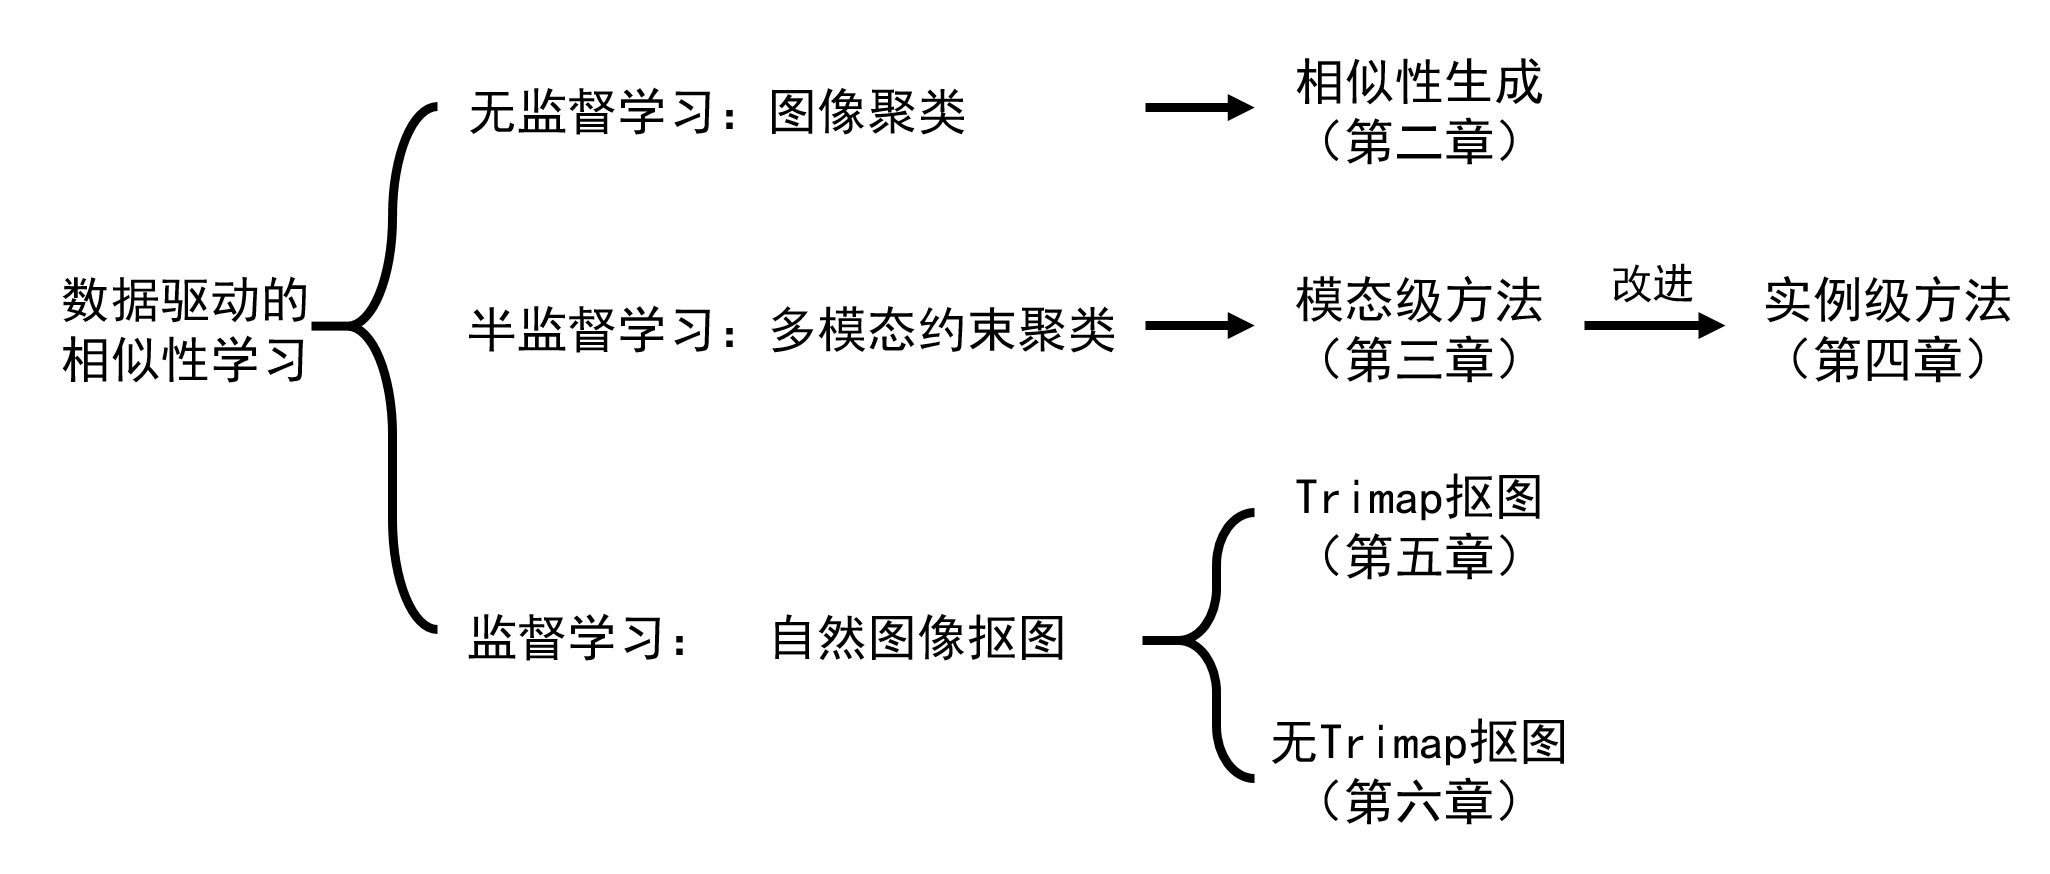
\includegraphics[width=0.9\columnwidth]{chap1/structure.png}
	\bicaption{全文结构示意图}{The structure of this thesis}
	\label{fig1:stru}
\end{figure} 